\documentclass[journal]{IEEEtran}
\usepackage[a5paper, margin=10mm, onecolumn]{geometry}
\usepackage{amsmath, amssymb}
\usepackage{bm}
\usepackage{graphicx}

% Define inner product notation
\newcommand{\innerproduct}[2]{\left\langle #1, #2 \right\rangle}

\begin{document}

\title{Matgeo : 2.6.12}
\author{AI25BTECH11006 - Nikhila}
\maketitle

\textbf{Problem:} Find the sine of the angle between the vectors $\vec{a}$ = $3\hat{i} + \hat{j} + 2\hat{k}$ and \\ \hspace*{1.3em} $\vec{b}$ = $2\hat{i} + -2\hat{j} + 4\hat{k}$
\vspace{1em}

\textbf{Solution:}

We know that
\[
\cos\theta = \frac{{a}\top {b}}{\|{a}\| \|{b}\|}.
\]

Calculating each term:

\begin{align}
{{a}}\top{{b}} &= 3(2) + 1(-2) + 2(4) = 6 - 2 + 8 = 12, \\
\|\vec{a}\| &= \sqrt{3^2 + 1^2 + 2^2} = \sqrt{14}, \\
\|\vec{b}\| &= \sqrt{2^2 + (-2)^2 + 4^2} = \sqrt{24}, \\
\cos\theta &= \frac{12}{\sqrt{14} \cdot \sqrt{24}} = \frac{12}{\sqrt{336}} = \frac{3}{\sqrt{21}}.
\end{align}

Now, to find \(\sin\theta\):

\begin{align}
\sin\theta &= \sqrt{1 - \cos^2\theta} \\
&= \sqrt{1 - \left(\frac{3}{\sqrt{21}}\right)^2} \\
&= \sqrt{1 - \frac{9}{21}} \\
&= \sqrt{\frac{12}{21}} \\
&= \frac{2}{\sqrt{7}}.
\end{align}

The sine of the angle between the vectors \(\vec{a}\) and \(\vec{b}\) is \(\frac{2}{\sqrt{7}}\).

\begin{figure}[ht!]
   \centering
   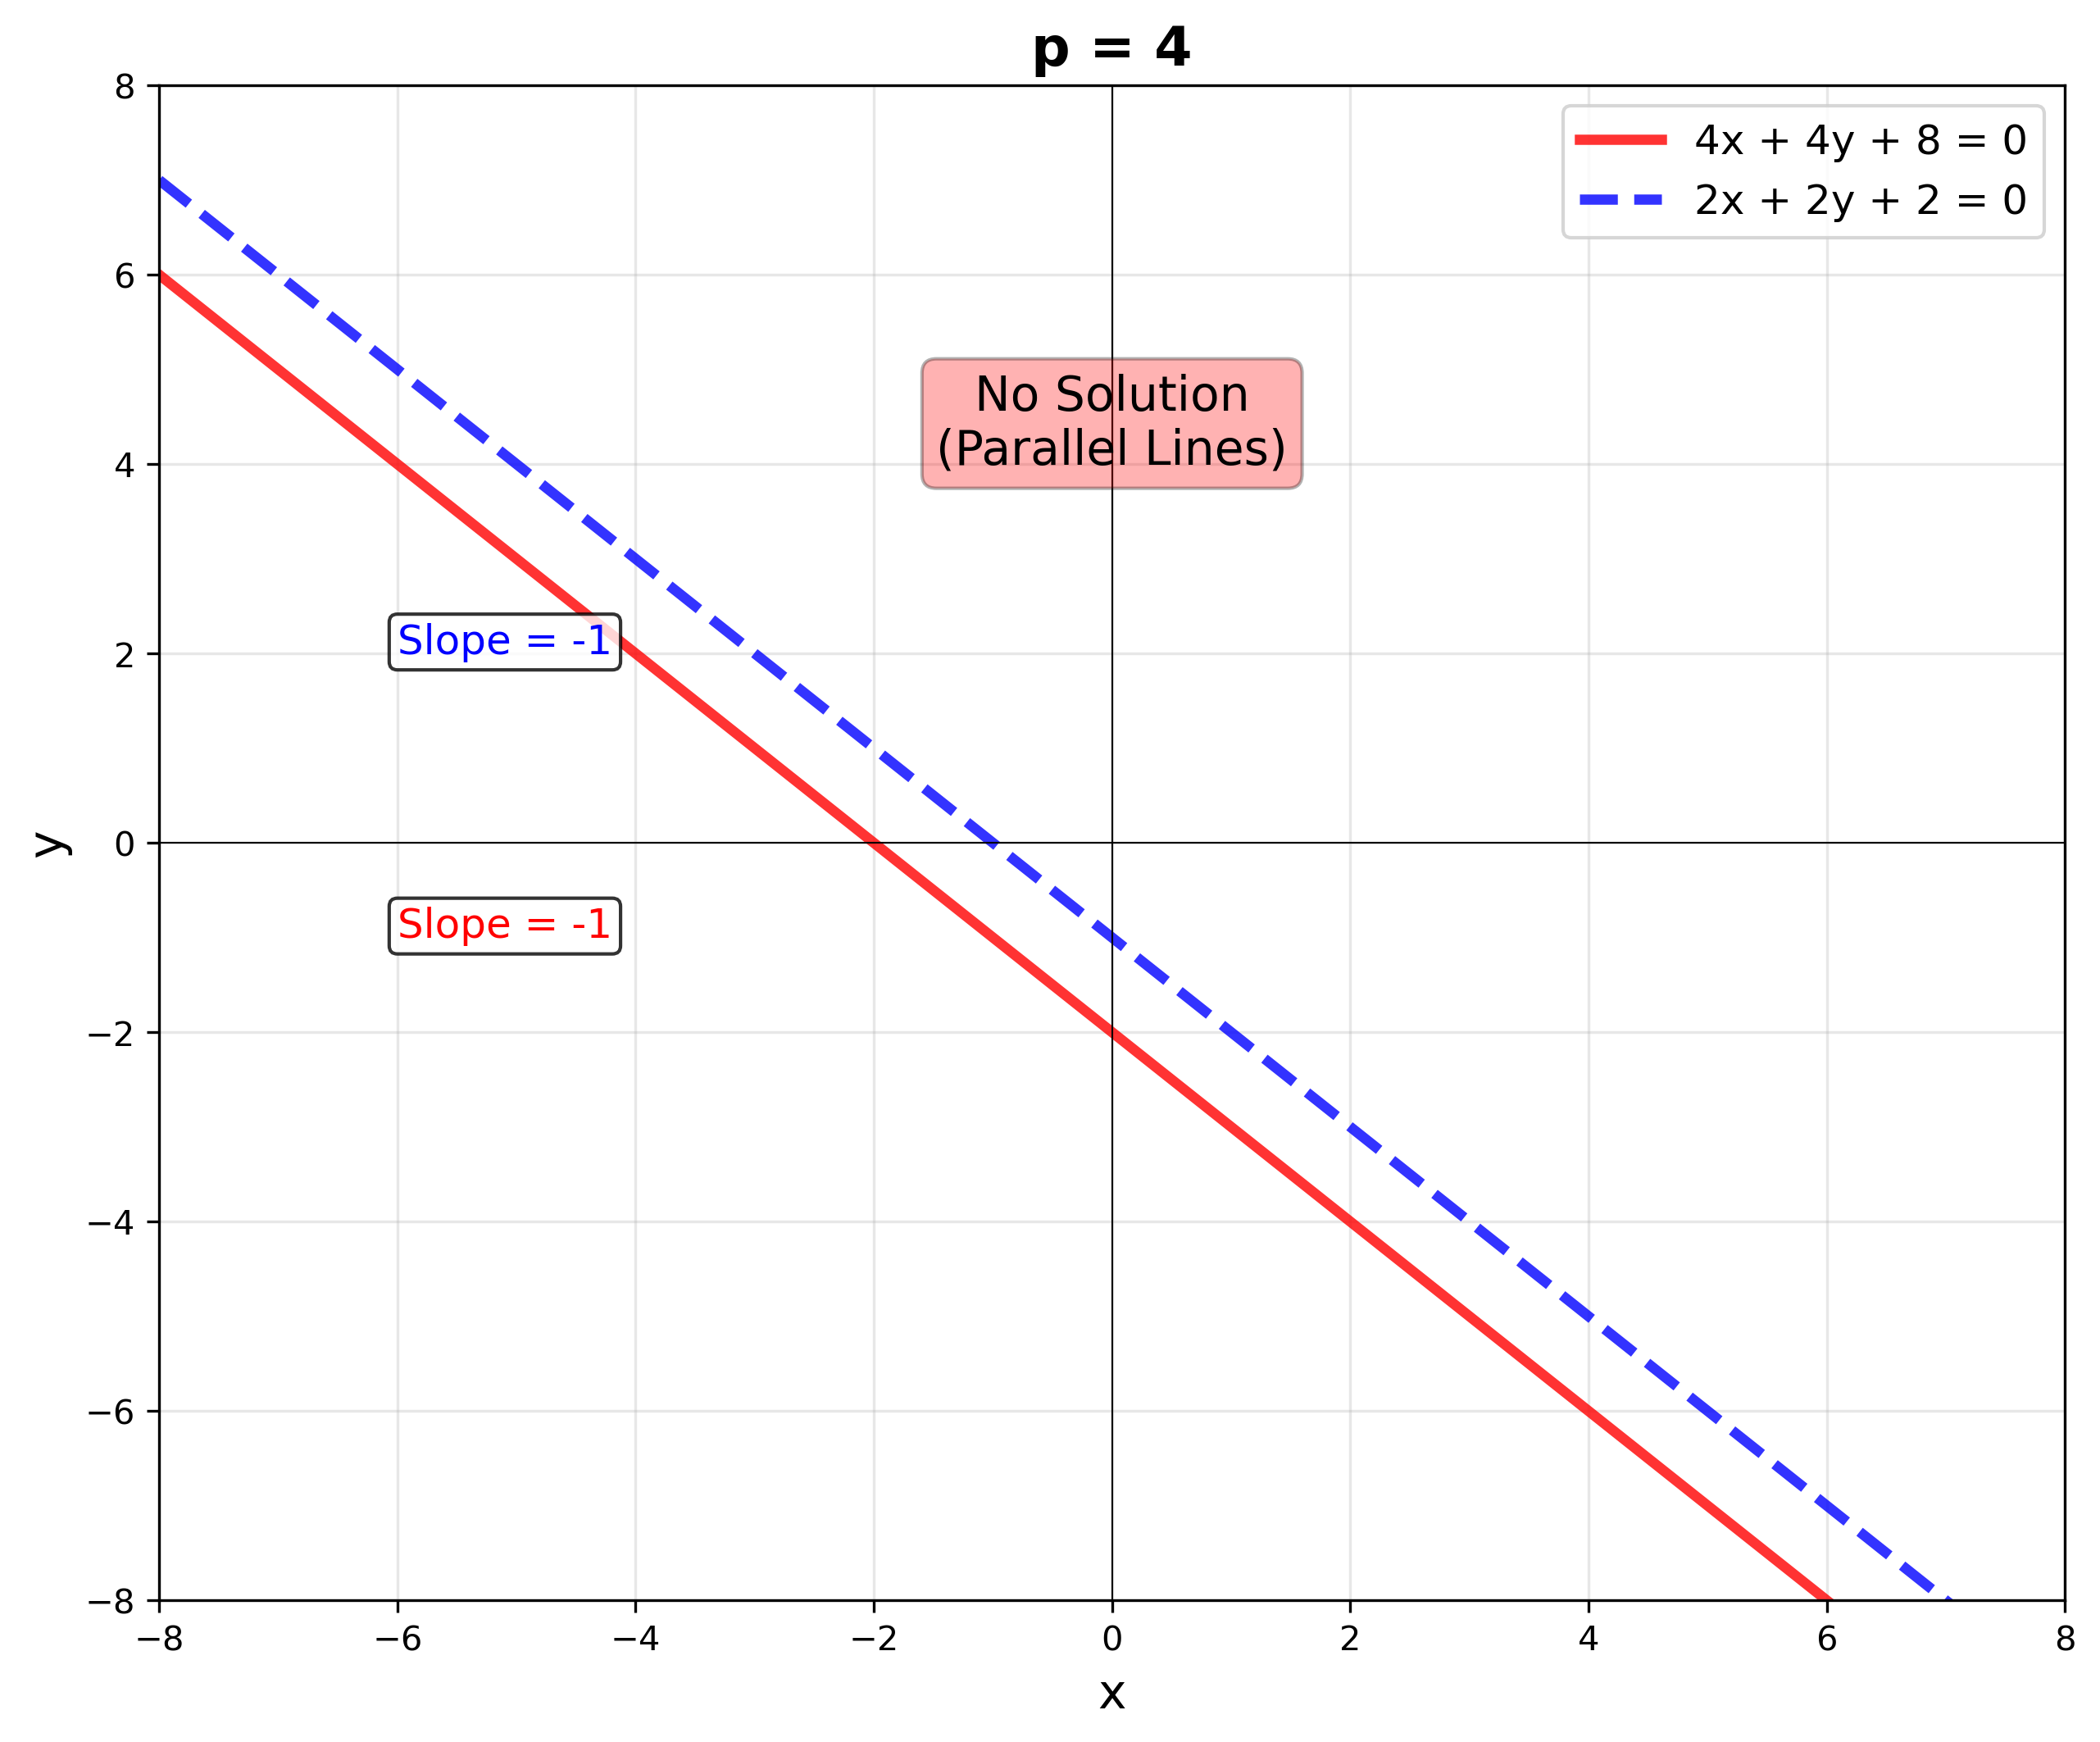
\includegraphics[width=1\linewidth]{fig1.png}
   \caption{}
   \label{}
\end{figure}



\end{document}

